%PREAMBOLO
\documentclass[a4paper, 12pt]{report}
\usepackage[italian]{babel}
\usepackage{graphicx}
\usepackage{amsmath,amssymb}
\usepackage{amsbsy}
\usepackage{xcolor}
\usepackage{enumitem}
\usepackage{multicol}
\usepackage{hyperref}
\usepackage{hyperref}
\hypersetup{
    colorlinks=true, %set true if you want colored links
    linktoc=all,     %set to all if you want both sections and subsections linked
    linkcolor=black,  %choose some color if you want links to stand out
}
\renewcommand{\footnoterule}{
  \kern -3pt
  \hrule width \textwidth height 1pt
  \kern 2pt
}%ALLUNGA LINEA PIE DI PAGINA
\setcounter{tocdepth}{3}%AGGIUNGE SUBSUBSECTION ALL'INDICE
%INIZIO
\begin{document}
\title{
\textbf{Cloud Green Computing}}
\author{Stefano Piccoli}
\date{\today}
\maketitle
\tableofcontents
\part{Cloud Computing}
    \chapter{IaaS (Infrastructure as a Service)}
      \section{Virtualizzazione}
        \paragraph{}La \textbf{virtualizzazione} rende possibile al sistema operativo di un server di eseguire su uno \textbf{strato virtuale} (\textbf{Hypervisor}).\\
        Questo permette di eseguire molteplici \textbf{macchine virtuali}, ognuna con il proprio sistema operativo, sullo stesso server fisico.
      \section{Hypervisor}
        \paragraph{}L'\textbf{hypervisor} crea lo strato di \textbf{virtualizzazione} che rende la virtualizzazione server possibile e contiene la \textbf{Virtual Machine Manager (VMM)}.
        \paragraph{Tipologie}
        \begin{itemize}
          \item \textbf{Type 1}: caricata direttamente sull'hardware, può eseguire più virtual server, usato per data center o server
            \subitem $\circ$ Hyper-v 
            \subitem $\circ$ ESX/ESXi 
            \subitem $\circ$ XenServer
          \item \textbf{Type 2}: caricata in un sistema operativo eseguito sull'hardware, greater overhead, usato per desktop e laptop
            \subitem $\circ$ Workstation 
            \subitem $\circ$ Virtual Server
            \subitem $\circ$ Fusion
        \end{itemize}
      \section{Amazon Elastic Compute Cloud 2 (EC2)}
      \begin{itemize}
        \item Mette a disposizione server virtuali (\textbf{istanze}) in modo semplice, veloce ed economico 
        \item Scelta tipo istanza e template da utilizzare (Windows/Linux) e numero istanze
        con AWS management console (o librerie SDK)
        \item \textbf{Opzioni di pagamento}: on demand, istanze riservate, istanze spot
        \item \textbf{Sicurezza} (Virtual Private Cloud - VPC
        \item \textbf{Storage persistente}: Amazon Elastic Block Store (EBS)
        \item \textbf{Autoscaling}
      \end{itemize}
      \section{Amazon Simple Storage Service (S3)}
      \begin{itemize}
        \item Fornisce uno \textbf{storage sicuro e facile} da usare
        \item Diverse \textbf{classi di memorizzazione} (standard / standard infrequent access / glacier)
        \item \textbf{Controllo} configurabile di \textbf{accesso ai dati}
      \end{itemize}
      \section{Amazon Elastic Block Store (EBS)}
      \begin{itemize}
        \item Blocco persistente di archiviazione di volumi di memoria usato con le istanze di Amazon EC2
        \item Ogni volume di Amazon EBS viene automaticamente replicato senza la sua Availability Zone in modo da offrire alta disponibilità e durata. 
      \end{itemize}
      \section{Dropbox exodus}
        \begin{itemize}
          \item I primi 8 anni della sua vita archiviava miliardi di file su Amazon S3
          \item Tra il 2014 e 2016 ha costruito la propria rete di server ideata dai propri ingegneri per spostare i dati
        \end{itemize}
        \subsection{L'esodo}
        \begin{itemize}
          \item Hardware proprietario che archivierà petabyte di dati
          \item Nuovo codice ("Magic Pocket")
          \item Installare 50 rack di hardware al giorno
          \item Completare lo spostamento prima della scadenza del contratto con Amazon per evitare un rinnovo
        \end{itemize}
        \subsection{Conclusioni}
        \paragraph{}Dropbox è riuscita a completare lo spostamento con successo entro i tempi previsti.
    \chapter{Container}
    \paragraph{}I \textbf{containers} sono un meccanismo di virtualizzazione differente dalle Virtual Machines poiché 
    permetto di avere più istanze \textbf{isolate} e \textbf{volatili} che scompaiono quando interrotte.\\
    I containers sono \textbf{leggeri}, \textbf{veloci}, più \textbf{semplici da buildare} ma \textbf{meno sicuri} delle Virtual Machines.
    \section{Docker}
    \paragraph{}\textbf{Docker} è un'azienda che ha realizzato una piattaforma che permette di \textbf{eseguire una applicazione in ambiente "isolato"}.\\
    Docker sfrutta la \textbf{virtualizzazione basata sui container} per eseguire in maniera isolata diverse \textbf{GUEST INSTANCES} sullo stesso sistema operativo.
    \subsection{Caratteristiche}
    \begin{itemize}
      \item \textbf{Portabilità}: il software può essere impacchettato in \textbf{images}, file read only che può essere mandato in esecuzione da docker e creare quindi il container
      \item Possono avere più istanze separate degli spazi utente (\textbf{containers})
      \item \textbf{Interfaccia} utente \textbf{semplificata}
      \item \textbf{Svantaggio}: sono meno isolati delle macchine virtuali, \textbf{condividono le risorse di sistema}
    \end{itemize}
    \subsection{Componenti}
    \begin{itemize}
      \item \textbf{Docker Engine}: permette di creare e mandare in esecuzione container
      \item \textbf{Docker Hub}: repository enorme che contiene molte immagini di container
      \item \textbf{Docker Swarm Mode}: permette di eseguire un container su più docker host e divide gli swarm node in manager e worker, permettendo una \textbf{gestione dichiarativa} della nostra \textbf{applicazione}
      \item \textbf{Images}: \textbf{template di sola lettura} usati per creare container, registrate in registry
      \subitem $\circ$ \textbf{Stratificazione}: ogni strato può essere a sua volta una immagine 
      \item \textbf{Registry}: \textbf{strutture di repository} che contengono insiemi di immagini per diverse versioni del sw
    \end{itemize}
    \subsection{Comandi}
    \begin{itemize}
      \item \textbf{PULL}: tiro un'immagine dal registry alla macchina
      \item \textbf{RUN}: viene creato il container dell'immagine
      \item \textbf{COMMIT}: salvare una nuova immagine
      \item \textbf{PUSH}: caricare una immagine nel registry
      \item \textbf{BUILD}: si crea un dockerfile che permette di creare un'immagine automaticamente
    \end{itemize}
    \subsection{Swarm mode}
    \begin{itemize}
      \item I nodi possono agire da \textbf{managers}, delegando tasks, o \textbf{workers}, eseguendo task assegnati.
      \item È possibile definire lo \textbf{stato dei vari servizi} nello stack dell'applicazione, incluso il numero di \textbf{task da eseguire in ogni servizio}
      \item \textbf{Swarm manager}:
        \subitem $\circ$ assegna ad ogni servizio nello swarm un unico DNS name
        \subitem $\circ$ bilancia il carico dei container in esecuzione 
        \subitem $\circ$ monitora lo stato del cluster e lo allinea con quello desiderato
    \end{itemize}
    \chapter{PaaS (Platform as a Service)}
      Servizio che fornisce hardware e software per lo sviluppo di applicazioni. L'utente deve fornire solo l'applicazione e i dati
    \paragraph{Vantaggi}
    \begin{itemize}
      \item Facilità di gestione e modifica dell'applicazione
      \item Facilità nell'adottare nuove tecnologie
    \end{itemize}
    \paragraph{Rischi}
    \begin{itemize}
      \item Disponibilità del servizio: l'interruzione del servizio da parte del fornitore comporta un immediato disservizio
      \item Vendor lock-in: difficoltà di cambiare servizio da parte del cliente
    \end{itemize}
      \section{Heroku}
      \paragraph{}\textbf{Heroku} è una piattaforma cloud basata su \textbf{container} con servizi integrati e un potente ecosistema che permette il deployment e running di applicazioni.
      \subsection{Dynos}
      \paragraph{}I \textbf{dynos} sono container Linux virtualizzati, Heroku trasforma l'applicazione utente in diversi \textbf{dynos}.
      \paragraph{Vantaggi}
      \begin{itemize}
        \item Scalabilità 
        \item Evitare di gestire l'infrastruttura
      \end{itemize}
      \paragraph{Premium:}
      \begin{itemize}
        \item \textbf{Scaling}
        \item \textbf{Autoscaling}: permette di inserire politiche per quando usare lo scaling
      \end{itemize}
      \subsection{Buildtime}
      \paragraph{}Per sviluppare una applicazione Heroku richiede:
      \begin{itemize}
        \item \textbf{Codice sorgente}
        \item \textbf{Lista di dipendenze}
        \item \textbf{Procfile}: file di testo che indica quale comando usare per far eseguire l'applicazione
      \end{itemize}
      Slug: Un insieme di codice sorgente, dipendenze, supporto per output, etc...
      Stack: Sistema operativo Ubuntu
      \subsection{Runtime}
      Nel \textbf{runtime} si prende lo slug e lo stack e vengono creati i dynos, che rappresentano le istanze utente, il dyno manager fa partire i container con il comando specificato dall'utente.
      \subsection{Esempio}
      \begin{enumerate}
        \item Applicazione riceve richiesta
      \end{enumerate}
      %SOTTO GRAFICO
      \subsection{Add-ons}
      \paragraph{}Gli \textbf{add-ons} sono funzionalità fornite da Heroku che possono essere aggiunte facilmente all'applicazione.
    \section{Altri PaaS}
    \begin{itemize}
      \item Microsoft Azure
      \item OpenShift
    \end{itemize}
  \chapter{Modelli di Business}
    \paragraph{}Un \textbf{business model} descrive il razionale di come una azienda \textbf{crea}, \textbf{consegna} e \textbf{acquisisce valore}.
    \begin{itemize}
      \item \textbf{Customer Segments}: il gruppo di persone o organizzazioni a cui il servizio mira di raggiungere
      \item \textbf{Valuer Propositions}: cosa rende speciale il servizio
      \item \textbf{Channels}: le modalità in cui la compagnia raggiunge il cliente
      \item \textbf{Customer Relationships}: tipo di relazione che la compagnia stabilisce col cliente 
      \item \textbf{Revenue Streams}: il flusso di entrate che la compagnia genera da ogni segmento di clientela
      \item \textbf{Key Resources}: le risorse più importanti richieste per il modello di business 
      \item \textbf{Key Activities}: le attività più importanti che la compagnia deve svolgere
      \item \textbf{Key Partners}: la rete di fornitori e partners per il business 
      \item \textbf{Cost Structure}: i costi che si incontrano per operare nel modello di business
    \end{itemize}
      \section{Business innovation}
        \begin{itemize}
          \item \textbf{Resource-driven}: ha origine da \textbf{infrastrutture o partner gia esistenti} usate per espandere o trasformare il business model 
          \item \textbf{Offer-driven}: crea nuova value proposition che influenza altri ambiti del business model
          \item \textbf{Custmer-driven}: basato sulle necessità del cliente, accesso facilitato o aumento di convenienza
          \item \textbf{Finance-driven}: guidata dal \textbf{revenue stream}, meccanismo di prezzi o riduzione dei cost structure
        \end{itemize}
  \part{Green Computing}
    \chapter{Introduzione}
    \paragraph{ICT è una minaccia per la sostenibilità ambientale?}
    \begin{itemize}
      \item La produzione di hardware produce inquinamento
      \item Gas serra
      \item e-waste
    \end{itemize}
    \paragraph{Green Computing}
    Pratica ambientale per calcolare la sostenibilità della computazione
    \begin{itemize}
      \item Minimizzare consumo energetico
      \item Progettare soluzioni efficienti energeticamente
      \item Riduzione e-waste
    \end{itemize}
      \section{Sprechi}
      \begin{itemize}
        \item 1,800 kg di materiale grezzo per produrre un personal computer (Rinoceronte)
        \item ICT contribuisce al 9\% di consumo elettrico in Europa 
        \item ICT contribuisce al 4\% di emissioni di carbonio in Europa
        \item Produce il 2\% delle emissioni di CO2 globali (carburante aereo)
        \item È previsto ulteriore aumento nei prossimi anni (esponenzialmente nel networking 20,9\%) 
        \item 50 milioni di tonnellate all'anno di e-waste (770 milioni di lavatrici)
        \item Il traffico di e-waste ha un traffico monetario illegale maggiore del traffico di droga
        \item  I data centre potranno arrivare al 28\% della domanda energetica per ICT.
      \end{itemize}
      \section{Datacenters}
      \begin{itemize}
        \item 40\% di consumo energetico per il raffreddamento
        \item PUE (Power Usage Effectiveness) $\frac{\text{Total Facility Power}}{\text{IT Equipment Power}}$ ma \textbf{non} misura la quantità di energia rinnovabile usata
      \end{itemize}
      \section{Obsolescenza programmata}
      Caratteristica di un prodotto volontariamente ideato per avere un "più breve" ciclo di vita.
      La vita del dispositivo deve durare abbastanza da soddisfare il cliente e fargli desiderare un nuovo dispositivo.
      \subsection{Cartello Phoebus}
      I più grandi produttori di lampadine si riunirono per accordarsi di produrre lampadine che durassero
      1000 ore invece di 2500 ore, anche se erano tutti in grado di produrre lampadine più longeve.
      \subsection{Obsolescenza percepita}
      Il cliente è convinto di aver bisogno di un prodotto aggiornato, anche se effettivamente quello attuale è perfettamente funzionante.
      \section{Progettare dispositivi efficienti energeticamente}
        \begin{itemize}
          \item Minimizzare processi di comunicazione, interazioni GUI-user
          \item Eliminare controlli non necessari
          \item Scegliere linguaggi di programmazione adatti
          \item Minimizzare movimenti di dati, usare efficacemente il caching
        \end{itemize}
    \chapter{Faas (Function As A Service)}
        \section{AWS Lambda}
          \begin{itemize}
            \item Eseguire codice senza fornire o gestire server, senza preoccuparsi dell'amministrazione
            \item Si occupa di scalare ed eseguire e patchare il codice
            \item È possibile impostare il codice in modo da attivarsi attraverso altri servizi AWS
            \item Pagamento solo per il tempo di calcolo
          \end{itemize}
        \clearpage
          \section{Tipi di FaaS:}
          \subsubsection{Commerciali}
          \begin{itemize}
            \item AWS Lambda
            \item Google Cloud Functions
            \item MS Azure Functions
          \end{itemize}
          \subsubsection{Open Source}
          \begin{itemize}
            \item Apache Openwhisk
            \item Fission
            \item Fn
            \item Knative
            \item Kubeless
            \item Nuclio
            \item OpenFaaS
          \end{itemize}
          \section{Due viste}
          \begin{figure}[h]
            \centering
            \includegraphics[scale=0.3]{Immagini/TwoViews.png}
          \end{figure}
          \section{Business View}
          \subsection{Business View: License}
            \begin{itemize}
              \item Opens Source: License permissive con Apache 2.0
              \item Commerciali: License proprietarie
              \item MS Azure Functions: anche progetti open sources
            \end{itemize}
            \begin{figure}[h]
              \centering
              \includegraphics[scale=0.4]{Immagini/License.png}
            \end{figure}
            \subsection{Business View: Installazione}
            \begin{itemize}
              \item Commerciali: Solo Azure ha alcune parti installabili in locale
              \item Piattaforme installabili supportano piu host, Kubernetes è il più supportato
            \end{itemize}
            \begin{figure}[h]
              \centering
              \includegraphics[scale=0.4]{Immagini/Installation.png}
            \end{figure}
            \clearpage
            \subsection{Business View: Source Code}
            \begin{itemize}
              \item Commerciali: MS Azure Function è l'unica parzialmente open source
              \item Open Source: Hostate su GitHub e implementate maggiormente in Go
            \end{itemize}
            \begin{figure}[h]
              \centering
              \includegraphics[scale=0.4]{Immagini/SourceCode.png}
            \end{figure}
            \subsection{Business view: Interface}
            \begin{itemize}
              \item Tutte le piattaforme forniscono CLI
              \item API e GUI non sempre fornite
            \end{itemize}
            \begin{figure}[h]
              \centering
              \includegraphics[scale=0.35]{Immagini/Interface.png}
            \end{figure}
            \clearpage
            \subsection{Business view: Community}
            \begin{itemize}
              \item OpenFaaS, Apache Openwhisk e Knative hanno la valutazione più alta su GitHub in stelle, contributors e commits rispettivamente
              \item Stackoverflow mostra un drastica differenza tra commerciali e open sources
            \end{itemize}
            \begin{figure}[h]
              \centering
              \includegraphics[scale=0.3]{Immagini/Community.png}
            \end{figure}
            \subsection{Business view: Documentation}
            \begin{itemize}
              \item Tutte le piattaforme forniscono deployment dell'applicazione e documentazione d'uso della piattaforma 
              \item Platform development e architettura non sono sempre documentate in piattaforme open sources
            \end{itemize}
            \begin{figure}[h]
              \centering
              \includegraphics[scale=0.3]{Immagini/Documentation.png}
            \end{figure}
            \clearpage
            \section{Technical View}
            \subsection{Technical view: Development}
            \begin{itemize}
              \item Java, Node.js e Python sono i piu supportati runtimes, Docker è inoltre popolare per personalizzazione runtime. 
              \item IDEs e text editor sono principalmente offerti dalle piattaforme \textbf{commerciali}.
            \end{itemize}
            \begin{figure}[h]
              \centering
              \includegraphics[scale=0.35]{Immagini/Development.png}
            \end{figure}
            \subsection{Technical view: Versioning}
            \begin{itemize}
              \item Open source: versioning implicito
              \item Commerciali: versioning dedicato
            \end{itemize}
            \begin{figure}[h]
              \centering
              \includegraphics[scale=0.5]{Immagini/Versioing.png}
            \end{figure}
            \subsection{Technical view: Function Orchestration}
            \begin{itemize}
              \item Tutte le piattaforme supportano invocazioni di funzioni HTTP-based \textbf{sincrone}, le \textbf{asincrone} invece da poche piattaforme
              \item Piu della metà delle piattaforme open source non supporta data store event sources
              \item Scheduler, stream processing platforms e messaging sono supportate dalla maggior parte delle piattaforme
              \item Più di metà delle piattaforme permette di integrare sorgenti di eventi custom
            \end{itemize}
            \begin{itemize}
              \item Più della metà dei FaaS supporta function orchestration usando altre DSLs o orchestrating functions.
            \end{itemize}
            \begin{figure}[h]
              \centering
              \includegraphics[scale=0.4]{Immagini/FunctionOrchestration.png}
            \end{figure}
            \subsection{Technical view: Testing \& debugging}
            \begin{itemize}
              \item La maggior parte delle piattaforme viste supporta testing funzionale e debug delle funzioni
              \item Commerciali: offrono operazioni più sofisticate
              \item Open Sources: test calls e log-based debugging
            \end{itemize}
            \clearpage
            \subsection{Technical view: Observability}
            \begin{itemize}
              \item Commerciali: tool dedicati al monitoraggio e logging
              \item Open source: richiedono integrazione di tool di terze parti
            \end{itemize}
            \begin{itemize}
              \item Più della metà dei FaaS supporta function orchestration usando altre DSLs o orchestrating functions.
            \end{itemize}
            \begin{figure}[h]
              \centering
              \includegraphics[scale=0.3]{Immagini/Observability.png}
            \end{figure}
            \subsection{Technical view: Application Delivery}
            \begin{itemize}
              \item La maggior parte delle piattaforme segue un approccio dichiarativo al deployment automatico delle applicazioni
              \item Commerciali: supportano nativamente CI/CD tool
              \item Open sources: Solo OpenFaaS integra CI/CD, le altre no
            \end{itemize}
            \begin{itemize}
              \item Più della metà dei FaaS supporta function orchestration usando altre DSLs o orchestrating functions.
            \end{itemize}
            \begin{figure}[h]
              \centering
              \includegraphics[scale=0.3]{Immagini/ApplicationDelivery.png}
            \end{figure}
            \subsection{Technical view: Application Delivery}
            \begin{itemize}
              \item La maggior parte delle piattaforme segue un approccio dichiarativo al deployment automatico delle applicazioni
              \item Commerciali: supportano nativamente CI/CD tool
              \item Open sources: Solo OpenFaaS integra CI/CD, le altre no
            \end{itemize}
            \begin{itemize}
              \item Solo AWS Lambda e MS Azure Functions sono affiliati a un function marketplace
            \end{itemize}
            \subsection{Technical view: Application Delivery}
            \begin{itemize}
              \item La maggior parte delle piattaforme segue un approccio dichiarativo al deployment automatico delle applicazioni
              \item Commerciali: supportano nativamente CI/CD tool
              \item Open sources: Solo OpenFaaS integra CI/CD, le altre no
            \end{itemize}
            \subsection{Technical view: Code Reuse}
            \begin{itemize}
              \item Solo AWS Lambda e MS Azure Functions sono affiliati a un function marketplace
            \end{itemize}
            \subsection{Technical view: Access Management}
            \begin{itemize}
              \item Commerciali: supportano nativamente autenticazione e controllo di accesso alle risorse 
              \item Open Source: usano funzioni offerte dal ambiente di hosting per garantire autenticazione e accesso alle risorse
            \end{itemize}
            \clearpage
            \section{FaaS Market}
            \begin{figure}[htbp]
              \centering
              \includegraphics[scale=0.5]{Immagini/FaasMarket.png}
              \includegraphics[scale=0.5]{Immagini/FaasMarket2.png}
            \end{figure}
      \chapter{Software sostenibile}
          \section{Nozioni di base}
          Efficienza: $$\varepsilon = \frac{\text{num.calcoli}}{\text{elettricità}}$$
          $\text{Efficienza} \neq \text{Correttezza}$\\[5px]
          \textbf{Sostenibilità}: Lo sviluppo sostenibile è lo sviluppo in grado di soddisfare i bisogni
          del presente senza compromettere la possibilità delle future
          generazioni di soddisfare i propri.
          \paragraph{Impronta ecologica massima consentita secondo l’accordo?} 2000 kg CO2 annui per persona.
          \paragraph{Quanta CO2 produce un cittadino europeo ogni anno?} 10000 kg.
          \paragraph{Quanto CO2 produce l’invio di una mail?} 20 g.
          \paragraph{Quanta CO2 produce una ricerca sul web?} 1 g.
          \paragraph{Ingegnere del software} Persona che applica i principi dell'ingegneria del software per progettare, sviluppare, mantenere,
          testare e valutare il software informatico.
          \section{Triangolo di ferro}
          \paragraph{}Gli ingegneri del software devono perseguire questi obiettivi contrastanti continuamente: \textbf{costo}, \textbf{tempo}, \textbf{qualità}.
          \section{Il modello Greensoft}
          \paragraph{}Il modello \textbf{Greensoft} è un modello olistico per lo sviluppo, utilizzo e dismissione di software sostenibile.
          \begin{figure}[htbp]
            \centering
            \includegraphics[scale=0.4]{Immagini/Greensoft.png}
          \end{figure}
          \section{Ruoli e collaborazione}
          \begin{itemize}
            \item Diversi ruoli possono essere ricoperti da una stessa persona
            \item Ruoli ricoperti da persone diverse necessitano collaborazione tra queste
            \item \textbf{DevOps fonde i ruoli di sviluppatore, operatore e architetto}
          \end{itemize}
          \section{Caso di studio}
          \subsection{Architetto}
          \paragraph{}Gli \textbf{architetti} sono coloro che determinano i requisiti funzionali e non-funzionali del sistema e che progettano le interazioni tra componenti.
          \begin{itemize}
            \item Possono includere la sostenibilità nei requisiti non-funzionali:
            \subitem $\circ$ \textbf{Scalabilità}: possibilità di adattare il sistema alla domanda
            \subitem $\circ$ \textbf{Performance}: tempo di risposta nel Service Level Agreement
            \item Come?
            \subitem $\circ$ scomponendo i servizi in \textbf{unità scalabili} (per risorsa: calcolo, rete, storage)
            \subitem $\circ$ rendere possibile un \textbf{bin packing} ottimo sull'utilizzo delle risorse di calcolo
          \end{itemize}
          \subsection{Bin packing}
          \begin{itemize}
            \item Problema difficile: \textbf{NP-hard}
            \item Corrisponde a minimizzare il numero di server per far girare i servizi che compongono il sistema
            \item L’architetto può disegnare componenti più piccole che consentono di risolvere il problema del bin packing evitando frammentazione
            \item La soluzione del problema verrà poi delegata a livelli più bassi gestiti da altri ruoli 
          \end{itemize}
          \subsection{CDN 101}
          \paragraph{}Mantenere i dati in punti di presenza locali:
          \begin{itemize}
            \item Minor distanza per raggiungere i dispositivi dei clienti
            \item Minore utilizzo di banda
            \item Miglior utilizzo della rete, mantenendo contenuti popolari in cache
          \end{itemize}
          \subsection{Scelte implementative}
          \begin{itemize}
            \item Implementare servizi che richiedano un quantitativo ragionevole di risorse anche per favorire \textbf{bin packing}
            \item Disaccoppiare implementazione da infrastruttura in modo da facilitare la migrazione a Cloud provider differenti
          \end{itemize}
          \subsection{Scegliere un linguaggio}
          \paragraph{}Trovare un bilanciamento tra \textbf{energia consumata}, \textbf{tempo di esecuzione} e \textbf{memoria utilizzata}.
          \begin{figure}[h]
            \centering
            \includegraphics[scale=0.5]{Immagini/Linguaggi.png}
          \end{figure}
          \subsection{Sviluppatore}
          \begin{itemize}
            \item Può cercare di ottimizzare l'efficienza del software 
            \item Disaccoppiare applicazione da dettagli sull'infrastruttura
            \item Ridurre lo spreco di risorse durante lo sviluppo
          \end{itemize}
          \subsection{Operatore}
          \paragraph{}Coloro che gestiscono l’infrastruttura e garantiscono la disponibilità dell’applicazione
          \begin{itemize}
            \item Offrono risorse infrastrutturali adeguate a garantire le performance desiderate
            \item Utilizzano al meglio le risorse per contenere i costi e favorire la sostenibilità
            \item Garantiscono backup e ripristino
            \item Implementano logs e monitoraggio
            \item Ottimizzare l’uso delle risorse
            \item Fare scelte infrastrutturali che garantiscano performance e facilitino il bin packing
          \end{itemize}
          \section{Quadro normativo}
          \begin{itemize}
            \item Le leggi e i regolamenti possono favorire una transizione sostenibile
            \item Le emissioni dovute al ciclo di vita di un software sono una esternalità negativa
            \item E’ un costo indiretto che viene pagato da terzi non coinvolti nel ciclo di vita di quel software
            \item Le leggi possono tassare le esternalità negative 
            \item Le leggi possono obbligare alla trasparenza per creare consapevolezza tra i clienti
          \end{itemize}
          \section{EU vs the World}
          \paragraph{}L’Unione Europea ha definito una direttiva su «Corporate sustainability reporting», all’interno del Green Deal europeo.
          \begin{itemize}
            \item Obbliga le aziende a relazionare sulla sostenibilità ambientale, sarà in vigore dal 2023.
          \end{itemize}
      \chapter{Microservizi}
          \paragraph{}Un \textbf{microservizio} ha l'obiettivo di accorciare il \textit{lead time} per nuove funzionalità e aggiornamenti. 
          \begin{itemize}
            \item Accelera il rebuild e il redeployment
            \item Riduce corde fra silos funzionali (vari gruppi di un'azienda)
            \item Riuscire a scalare efficacemente
          \end{itemize}
          \paragraph{Svantaggi}
          \begin{itemize}
            \item Eccesso di comunicazione
            \item Complessità
            \item Difficoltà nell'evitare duplicazione dei dati 
          \end{itemize}
          \section{Monoliti}
          \paragraph{}Per \textbf{monolite} si intende la tipica applicazione di un'azienda il quale cambiamento di una piccola parte richiede
          il \textbf{rebuilding} e il \textbf{redeployment} dell'intero monolite. Inoltre lo \textbf{scaling} è richiesto per l'intera applicazione.
          \section{Microservizi}
          \subsection{Service-orientation}
            \paragraph{}Sviluppare un'applicazione come un insieme di servizi
            \begin{itemize}
              \item Ogni servizio è eseguito in container separati
              \item Comunicazione con meccanismi leggeri (HTTP request-response e code asincrone per disaccoppiamento)
              \item Poliglotta (linguaggi diversi)
            \end{itemize}
          \subsection{Organizzare servizi intorno alle business capability}
            \begin{itemize}
              \item Cross-functional team
            \end{itemize}
          \subsection{Decentralizzazione dei dati}
          \begin{itemize}
            \item Ogni servizio ha un suo database
            \item Eventual consistency e compensation invece di transazioni distribuite
          \end{itemize}
          \subsection{Servizi sviluppabili indipendentemente}
          \begin{itemize}
            \item Possibilità di modificare il servizio senza necessariamente cambiare gli altri servizi
          \end{itemize}
          \subsection{Servizi scalabili in orizzontale}
          \begin{figure}[htbp]
            \centering
            \includegraphics[scale=0.3]{Immagini/HScaling.png}
            \includegraphics[scale=0.3]{Immagini/HVScaling.png}
          \end{figure}
          \subsection{Servizi resistenti agli errori}
          \begin{itemize}
            \item Tolleranza agli errori è un requisito
            \item Ogni chiamata di servizio può fallire 
            \item Chiamate sincrone tra servizi possono indurre a problemi di downtime
          \end{itemize}
        \section{CAP Theorem}
        \paragraph{}In presenza di una \textbf{partizione} di rete, non puoi avere sia \textbf{accessibilità} che \textbf{consistenza}.
        \subsection{Approccio Netflix}
        \paragraph{}Per replicare i dati in \textit{n} nodi Netflix:
        \begin{itemize}
          \item Scrive dove è momentaneamente possibile, poi sistema le mancanze
          \item Usa il quorum: (n/2+1) devono rispondere
        \end{itemize}
        \section{Chaos monkey}
        \paragraph{}Il metodo \textbf{chaos monkey} termina casualmente istanze e container che vengono eseguiti all'interno dell'ambiente di produzione
      \chapter{Kubernetes}
        \section{Containers}
        \begin{itemize}
          \item I container forniscono un meccanismo leggero per isolare lo l'ambiente di un'applicazione
          \item Le immagini dei container possono essere eseguiti in modo affidabile su ogni macchina, fornendoci la portabilità dallo sviluppo al deployment
          \item Più carichi di lavoro possono essere piazzati sulla stessa macchina fisica, raggiungendo elevati utilizzi di memoria e CPU
        \end{itemize}
        \section{Kubernetes (Container Orchestration)}
          \begin{itemize}
            \item Gestisce l'intero ciclo di vita dei singoli container, \textbf{avviando o spegnendo le risorse in base alla necessità}.
            Se un container si spegne inaspettatamente K8 ne lancia un altro al suo posto.
            \item Fornisce un \textbf{meccanismo} alle applicazioni per \textbf{comunicare tra loro} anche quando i container sottostanti vengono creati e distrutti.
            \item Dato un gruppo di carichi di lavoro per container da eseguire e un insieme di macchine su un cluster, esamina ogni container e \textbf{determina la macchina ottimale
                  a cui schedulare il carico di lavoro}
          \end{itemize} 
        \clearpage
          \section{Design principles: Dichiaratività}
          \paragraph{} K8s troverà quando l'attuale stato del sistema non rispetta le nostre aspettative e interverrà per sistemare il problema (\textbf{self-healing}).
          \paragraph{Definiamo gli stati desiderati da una collezione di oggetti}
          \begin{itemize}
            \item Ogni oggetto ha una specifica nella quale forniamo lo stato desiderato e uno stato che riflette lo stato corrente dell'oggetto
            \item K8 esegue costantemente domande a ogni oggetto per assicurarsi che il suo stato sia uguale alla specifica
            \subitem{$\circ$} Se un oggetto non risponde, K8 avvia una nuova versione per sostituirlo
            \subitem{$\circ$} Se un oggetto si è allontano dalle specifiche, K8 emette i comandi necessari per riportare l'oggetto allo stato desiderato
          \end{itemize}
          \section{Design principles: Distribuzione}
          \paragraph{}K8s fornisce una interfaccia unificata per interagire con un cluster di macchine. Non ci dobbiamo preoccupare della comunicazione tra le singole macchine.
          \begin{figure}[htbp]
            \centering
            \includegraphics[scale=0.4]{Immagini/k8distribuzione.png}
          \end{figure}
          \clearpage
          \section{Design principles: Disaccoppiamento}
          \begin{itemize}
            \item I container dovrebbero essere sviluppati avendo un solo obiettivo in mente (\textbf{microservice-based architecture})
            \item K8s supporta nativamente l'idea di disaccoppiare i \textbf{servizi} che possono essere \textbf{scalati e aggiornati indipendentemente}
          \end{itemize} 
          \section{Design principles: Strutture immutabili}
          \begin{itemize}
            \item Per ottenere il massimo dai container e dall'orchestrazione, dovremmo distribuire una \textbf{struttura immutabile}
            \item Durante il ciclo di vita di un progetto dovremmo \textbf{usare la stessa immagine per il container} (e modificare solo le configurazioni esterne all'immagine)
            \item I container sono progettati per essere \textbf{effimeri}, \textbf{pronti per essere rimpiazzati da altri container} in qualsiasi momento
            \item Mantenendo la struttura immutata rendiamo più facile il \textbf{roll back} delle applicazioni \textbf{a stati precedenti}, possiamo semplicemente aggiornare la nostra configurazione per usare una vecchia immagine del container.
          \end{itemize}
          \clearpage
          \section{K8s Objects}
          \paragraph{}Gli oggetti di K8s possono essere definiti in \textbf{manifesti} (YAML o JSON).
          \subsection{K8s objects: Pod}
          \paragraph{}Un \textbf{Pod} consiste in 
            \begin{itemize}
              \item uno o più container strettamente in relazione
              \item un livello di rete condiviso
              \item un volume di filesystem condiviso
            \end{itemize}
          \subsection{K8s objects: Deployment}
          \paragraph{}Un \textbf{deployment} object include una collezione di \textbf{Pods} definiti da un template e il numero di copie del template che si vogliono eseguire.
          Il cluster proverà sempre ad avere n Pods disponibili.
          \begin{figure}[h]
            \centering
            \includegraphics[scale=0.5]{Immagini/Deployment.png}
          \end{figure}
          \clearpage
          \subsection{K8s objects: Service}
          \paragraph{}Ogni Pod è assegnato ad un unico indirizzo IP che possiamo usare per comunicare con esso.\\
          \textbf{Service} fornisce un endpoint stabile per direzionare il traffico al Pod desiderato anche se il Pod subisce aggiornamenti, scaling o failures.
          \begin{figure}[h]
            \centering
            \includegraphics[scale=0.3]{Immagini/Service.png}
          \end{figure}
          \subsection{K8s objects: Ingress}
          \paragraph{}Per esporre la nostra applicazione a traffico esterno verso il nostro cluster, definiamo un \textbf{Ingress} object.
          \begin{figure}[h]
            \centering
            \includegraphics[scale=0.35]{Immagini/Ingress.png}
          \end{figure}
          \section{K8s Control plane}
          \paragraph{}Ci sono due tipi di macchine in un cluster:
          \begin{itemize}
            \item \textbf{Master node}: macchina che contiene la maggior parte dei componenti del control plane
            \item \textbf{Worker node}: macchina che esegue i workloads delle applicazioni0
          \end{itemize}
          \subsection{K8s Control plane: Master node}
          \paragraph{}L'utente fornisce nuovi object specification all'\textbf{API server} del master node:
          \begin{itemize}
            \item Il server API convalida le richieste di aggiornamento e agisce come interfaccia unificata per richieste sullo stato corrente del cluster
            \item Lo stato del cluster è archiviato in una key-value distribuita \textbf{etcd}
          \end{itemize}
          \paragraph{}Lo \textbf{scheduler} determina dove gli oggetti dovrebbero essere eseguiti. Lo scheduler:
          \begin{itemize}
            \item Richiede il server API i cui oggetti non sono stati assegnati ad una macchina
            \item Determina a quali macchine quegli oggetti dovrebbero essere assegnati
            \item Risponde all'API server di riflettere il compito
          \end{itemize}
          Il \textbf{controller-manager} monitora lo stato dei cluster attraverso i server API, se lo stato attuale differisce dallo stato desiderato, il \textbf{control manager} 
          effettuerà dei cambiamenti attraverso il server API per guidare il cluster verso lo stato desiderato.
          \subsection{K8s Control plane: Worker node}
          \paragraph{}\textbf{Kubelet}:
          \begin{itemize}
            \item Agisce come agente del nodo che comunica con il server API per vedere quali container workloads sono stati assegnati al nodo
            \item Responsabile di far eseguire i workload assegnati ai Pods
            \item Quando un nodo entra la prima volta in un cluster, annuncia l'esistenza del nodo al server API in modo che lo scheduler possa assegnare il Pod a esso
          \end{itemize}
          \paragraph{}\textbf{Kube-proxy} abilita i container a comunicare tra loro attraversando vari nodi sul cluster
          \section{Quando non usare K8s}
          \begin{itemize}
            \item Se puoi eseguire workload su una singola macchina
            \item Se i calcoli sono leggeri
            \item Se non necessiti alta disponibilità e puoi tollerare downtime
            \item Se non prevedi molte modifiche al servizio 
            \item Se hai un monolite e non prevedi di spezzarlo in microservizi
          \end{itemize}
          \section{K8s vs Docker Swarm}
          \begin{figure}[htbp]
            \centering
            \includegraphics[scale=0.35]{Immagini/K8svsDS.png}
          \end{figure}
          \chapter{Datacenters}
          \section{Google datacenter}
          \begin{itemize}
            \item Differenti livelli di sicurezza (badges, scanner biometrici)
            \item Distribuzione elettrica sospesa
            \item Armadi personalizzati
            \item Tecnologia di raffreddamento (27 gradi)
          \end{itemize}
          \section{Pisa datacenter}
          \begin{itemize}
            \item 100 Gbit/sec DCI (DataCenter Interconnect)
            \item No Single Point of Failure(SPOF): ridondanza a L3 e L2, collegamento fisico
            \item Spine-leaf topology per il traffico Est-Ovest
            \item San Piero datacenter: Raffreddamento adiabatico (PUE<1.3)
          \end{itemize}
          \section{Metodi di raffreddamento}
          \begin{itemize}
            \item \textbf{Evaporative coolers}: Più efficienti energeticamente dei sistemi a aria, richiedono grandi volumi di acqua e costi di mantenimento e trattamenti chimici
            \item \textbf{Air coolers}: Difficile raffreddamento durante l'estate e ha una costosa struttura di supporto
            \item \textbf{Adiabatic coolers}: Evaporative(periodi caldi) + Air(durante tutti gli altri periodi). Il sistema ad aria viene usato per circa l'85\% del tempo in un anno risparmiando il 90\% di acqua.
          \end{itemize}
          \section{DCIM: Data Center Infrastructure Management}
          \begin{itemize}
            \item Monitoraggio centralizzato di infrastrutture fisiche
            \subitem $\circ$ Power 
            \subitem $\circ$ Cooling 
            \subitem $\circ$ Security 
            \subitem $\circ$ Ambiente 
            \item Genera report e grafici basati sull'utente
            \item Notifica di errori istantanea consente una rapida risoluzione di eventi critici all'infrastruttura
          \end{itemize}
          \section{Cosa non fare in un datacenter}
          \begin{itemize}
            \item Grovigli di cavi, sono pericolosi
            \item Introdurre cibi e bevande
            \item Non avere documentazione dettagliata
            \item Non prevenire problemi elettrici
            \item Non tenere traccia degli accessi
            \item Non prevedere incendi
          \end{itemize}
          \section{Checklist}
          \begin{itemize}
            \item Garantisce qualità delle operazioni, indipendentemente dall'operatore
            \item Riduce la responsabilità degli impiegati
          \end{itemize}
          \section{BC/DR: Business Continuity e Disaster Recovery}
          \begin{itemize}
            \item Avere una copia dei tuoi dati più importanti fuori dall'ambiente di produzione (almeno 150 miglia)
            \item Un piano non testato e un piano fallito: Testa il tuo BC/DR in modo realistico per garantirne il funzionamento
            \item Assicurati che le modifiche alla produzione siano propriamente riflesse nel piano BC/DR
            \item Avere un piano consiste e accessibile anche in eventi di maggiore disastro
            \item Avere sempre professionisti allenati al piano BC/DR 
            \item Murphy's law: Se qualcosa può andare storto, lo farà
          \end{itemize}
          \section{Peggiori disastri nei datacenter}
          \begin{figure}[h]
            \centering
            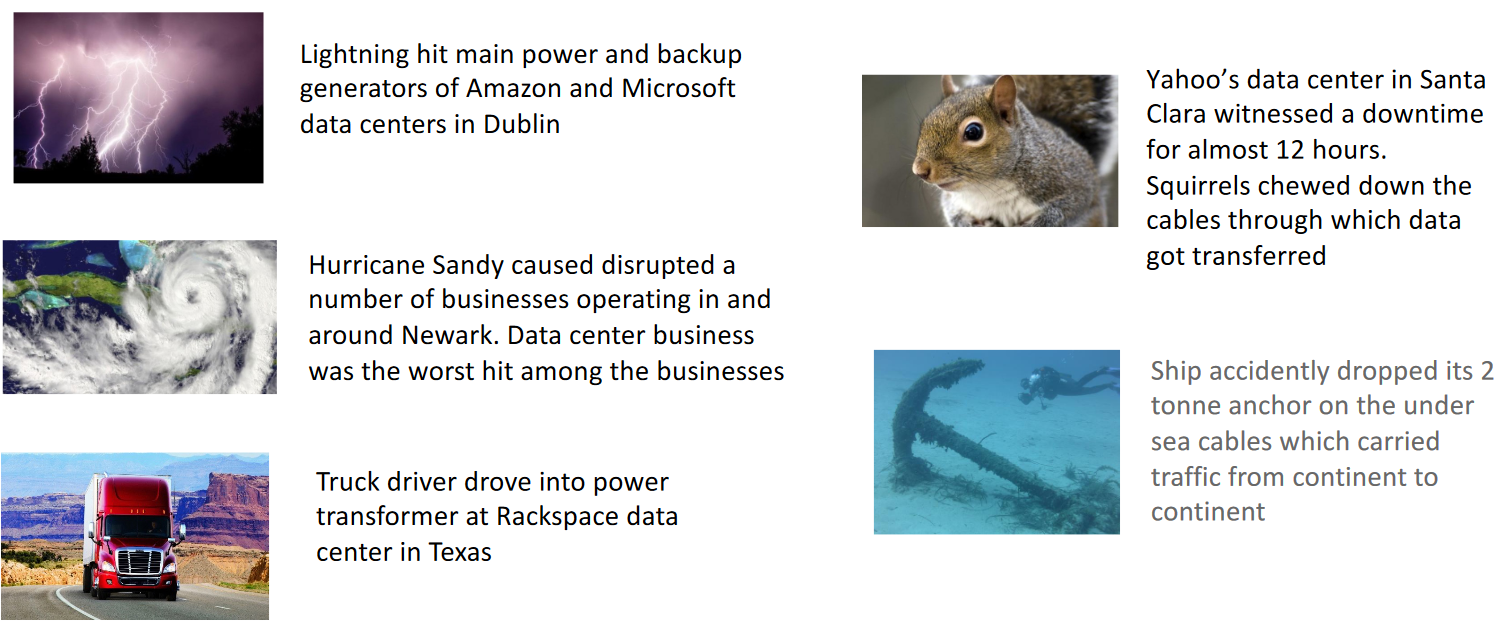
\includegraphics[scale=0.30]{Immagini/Disastri.png}
          \end{figure}
          \clearpage
          \section{Hyperconvergence - Iperconvergenza}
          \begin{itemize}
            \item Infrastrutture DC tradizionali 
            \subitem $\circ$ Server, networking e storage separati 
            \subitem $\circ$ Problemi: compatibilità dei componenti
            \item Infrastrutture convergenti
            \subitem $\circ$ Pre-testate, design validato
            \subitem $\circ$ Strumenti avanzati di gestione
            \item Iperconvergenze 
            \subitem $\circ$ Combina server virtualizzati, networking e storage in un singolo box
            \subitem $\circ$ Costi di hardware minimizzati e scalabilità
            \subitem $\circ$ Non può aumentare storage senza aumentare il calcolo
            \subitem $\circ$ Applicazioni DB non virtuali(No storage virtualizzato)
            \subitem $\circ$ Software NON economico
            \subitem $\circ$ \textbf{Nutanix} è stato nominato leader per iperconvergenza per il quinto anno di fila
          \end{itemize}
        \chapter{Internet of things}
        \section{Data usage}
        \begin{figure}[htbp]
          \centering
          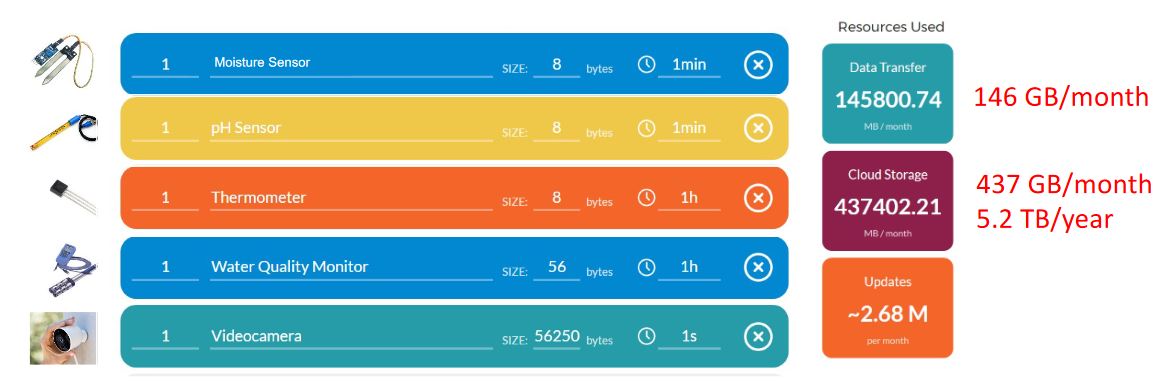
\includegraphics[scale=0.3]{Immagini/DataUsage.png}
        \end{figure}
        \section{Deployment models}
        \begin{figure}[htbp]
          \centering
          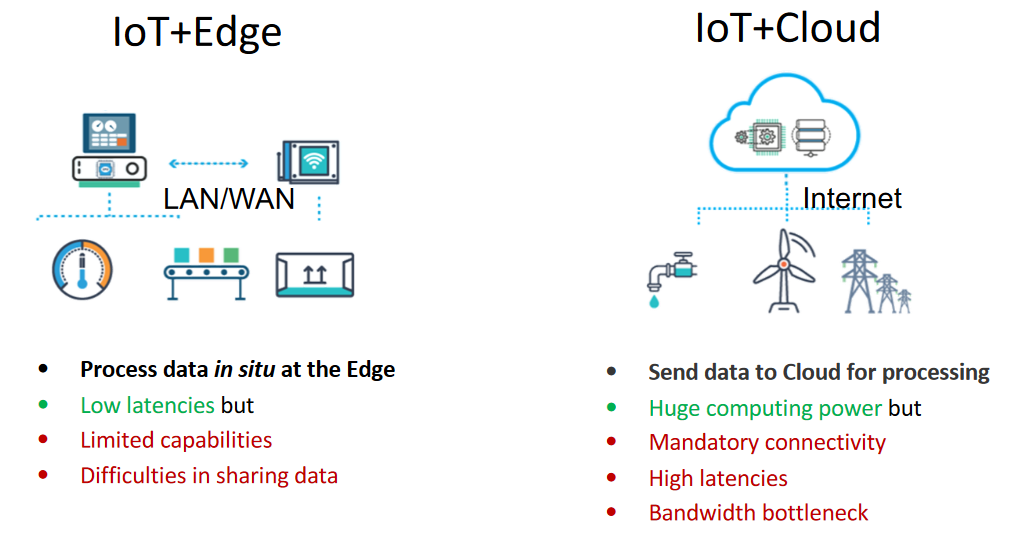
\includegraphics[scale=0.4]{Immagini/DeploymentModels.png}
        \end{figure}
        \section{Fog Computing}
        \paragraph{}\textbf{Fog computing} mira ad estendere il cloud attraverso IoT per supportare meglio le applicazioni IoT \textbf{latency-sensitive} e \textbf{bandwidth-hungry}.
        \section{Fog infrastructure}
        \begin{figure}[htbp]
          \centering
          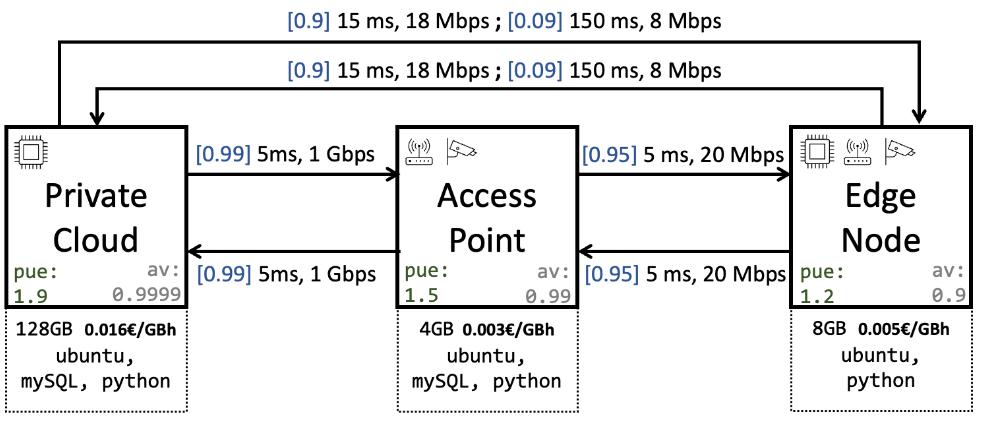
\includegraphics[scale=0.5]{Immagini/FogInfrastructure.png}
        \end{figure}
        \begin{itemize}
          \item Hardware, software, IoT capabilities
          \item Costi
          \item Disponibilità dei nodi
          \item $PUE=\frac{E_{IT}+E_{non-IT}}{E_{IT}}$
        \end{itemize}
\end{document}